%   Simulators for testing
%       + SITL, JSBSim, Flightgear, Simple GNSS
\subsection{Vehicle simulation}
    \todo{write about vehicle simulation}
    With software in the loop (SITL), ardupilot can be run without any hardware. The vehicle is simulated through a flight dynamics model (FDM) which communicates with a flight simulator. The flight simulator simulates measurements and dispatches these to ardupilot.\\
    
    
    \todo{
        Questions: 
        What is the default alternative to FG?
        What is the role of ardupilot in the simulator?
        Why is there a direct connection between FG and DUNE?
        Why does FG provide a better resolution for IMU?
        Including the FG task send measurements directly to AP-task?
        Is the precision lowered when it goes through AP?
        Is JSBsim the default FDM?
        Does Mavproxy and Neptus communicate?
    }
    Ardupilot is configured to work with the FDM JSBsim. It is cross platform and contains models for a range of different vehicles, although this implementation simply uses the default model of the Rascal110 RC plane. 
    
    \todo{Hva var alternativet til flightgear?}
    %\paragraph{JSBsim}
        %http://jsbsim.sourceforge.net/
        %http://wiki.flightgear.org/JSBSim
        %Bare bones system model that runs on multiple OS's
        %"Flight dynamics model"
        %is a cross platform flight dynamics model. It supports vehicles of many different kinds
    
    %\paragraph{Flightgear}
        %http://wiki.flightgear.org/Flightgear
        %Built on top of jsbsim. Adds a visual interface, cross platform
        %Flight simulator 
%        is a flight simulator running on top of a flight dynamics model, such as JSBsim. It has been used instead of the native ardupilot simulator because of its better IMU measurement precision.
    
%\subsection{ArduPilot Software In The Loop}
    %http://ardupilot.github.io/MAVProxy/html/index.html
    %Neptus, mavproxy, flightgear, gnss / rtklib playback file
%    With software in the loop (SITL), ardupilot can be run without any hardware. 

\subsection{GNSS}
    A simple GNSS simulator has been implemented in DUNE. The focus of the simulator is to provide pseudorange and doppler measurements to a receiver, and as such no ephemeris calculations are made for the simulated satellite positions or velocity. For simplicity the satellites are kept stationary with zero velocity. Positions are taken from a snapshot of visible GPS satellites in the Trondheim area at 13:00 the 13th of November 2018. A visibility plot shows the satellites with respect to elevation angle and azimuth in figure \ref{fig:visplot}.\\

    %Constellation of six stationary satellites with no noise or bias
    %Subscribes to ExternalNavData
    \begin{figure}[!htbp]
        \centering
        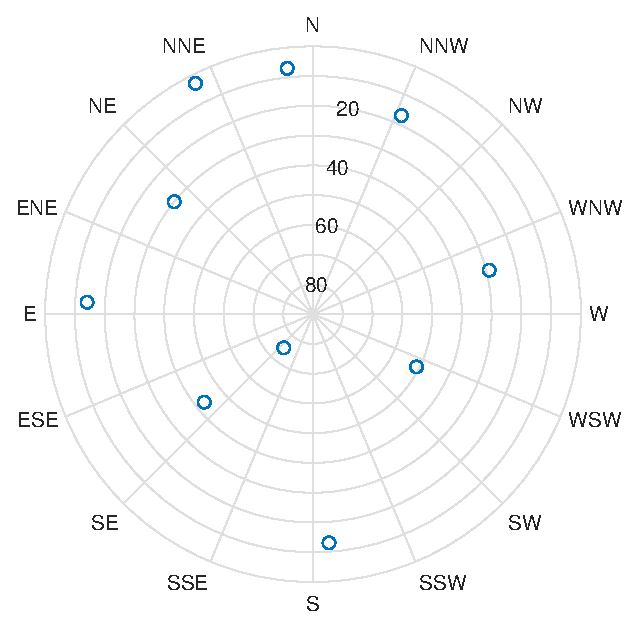
\includegraphics[scale=0.7]{Implementation/Images/visibilityplot.eps}
        \caption{Visibility plot of the satellites in the simulator from Trondheim. The user position is in the middle, while the dots denote satellites above the horizon. The distance between user and satellites in the plot is the given by the elevation angle. The angle from the north axis is the azimuth.}
        \label{fig:visplot}
    \end{figure}

    Each satellite of the simulator runs as a separate task on the system. The output of the tasks comes in the form of the IMC message RawGNSSdata, containing satellite position and range and doppler shift measurements. The input is another IMC message, ExternalNavData, containing the true state of the system, dispatched by the ardupilot task. As all the satellites in the constellation run as separate tasks, the true state will be received at the same time for all satellites. In other words, the satellites dispatch messages separately while sharing inputs. As a result, GNSS-messages will be dispatched approximately simultaneously, resulting in messages being sent in \textit{bursts}, resulting in an excessively small time step between measurements. This is not ideal for a discretized system and should be handled. Distinct delays between the satellite tasks are therefore introduced, which spread the dispatching of GNSS messages evenly. Another option would be to buffer the GNSS messages at the integration filter and run all measurements together, but this introduces an unnecessary layer of complexity for the filter. \\
    \todo{forsinkelse i posisjon mellom simulator og filter (noen pseudoranges blir feil/utdatert)}
    \todo{PX BBB 20 ms delay?}

\subsection{The full simulator}
    %Neptus and mavproxy
    \todo{write about full simulator}
    \todo{Dune bridges the connection between Neptus and ArduPilot by relaying setpoints and states}
    Neptus has the ability to interface with Ardupilot and can be used to control the simulated vehicle. Not only does this provide the operator with a visual interface for executing maneuvers, but it also offers extensive plotting functionality of messages from the IMC bus shared with DUNE. DUNE is also configured with the FlighGear task that provides a better resolution of IMU measurements than native arduplane.

    \begin{figure}
        \centering
        \includegraphics[scale=0.8]{Images/Simulator.pdf}
        \caption{Simulator block diagram}
        \label{fig:sim-diag}
    \end{figure}
%\includepdf[pages=-]{Images/sim_diagram.pdf}
%\includepdf{Images/sim_diagram.pdf}
%SIM_VEHICLE: "mavproxy.py" "--master" "tcp:127.0.0.1:5760" "--sitl" "127.0.0.1:5501" "--out" "127.0.0.1:14550" "--out" "127.0.0.1:14551" "--map" "--console"
%flightgear: 5503
%ntnu-x8-001 on AP serial 2
%dune task: tcp:5760
